We have access to data from a randomized trial~(rct) and an observational study~(os), which come from an underlying distribution $\pfull^\diamond$ 
over $\left(X, U, Y(0), Y(1),Y, T\right)$, for $\diamond \in  \{\rct,\obs\}$. Here, $\left(X, U\right) \in \RR^\xdim \times \RR^\udim$ is a vector of confounders, $\left(Y(0), Y(1)\right)$ are real-valued bounded potential outcomes, $Y \in \RR$ is the observed outcome, and $T \in \{0,1\}$ is a binary treatment 
indicator. However, the confounder $U$ and the potential outcomes are never observed, that is, we can only sample from the distributions $\prct \defeq \margin(\pfullrct)$ and $\pobs \defeq \margin(\pfullobs)$, where $\margin(\pfull)$ denotes the marginal distribution of $(X,Y,T)$ under $\pfull$.

\begin{wrapfigure}{r}{0.4\textwidth} 
\vspace{-5mm}
\begin{center}
    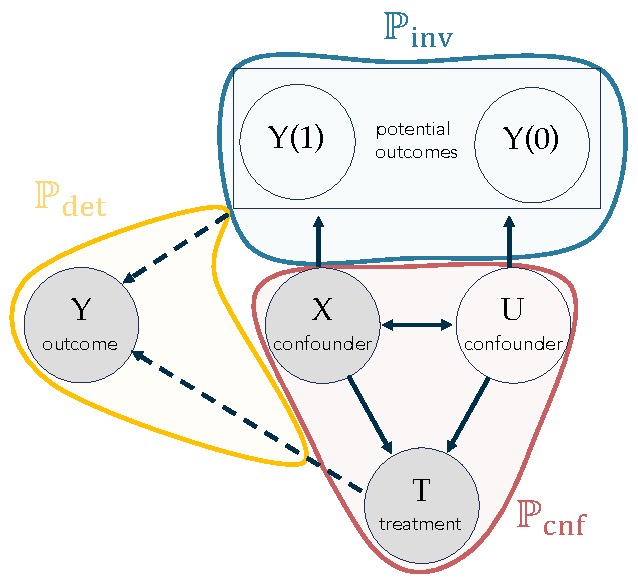
\includegraphics[width=0.4\textwidth]{dag}
  \end{center}
  \caption{Graphical model that captures the Neyman-Rubin potential outcome framework with unobserved confounder $U$. $\pinv$ is the causal mechanism that does not change between the randomized trial and the observational study, while $\pconf$ changes across studies. 
  For the randomized trial, we assume there is no arrow from the confounders ($X, U$) to the treatment indicator $T$ due to its internal validity. 
  Observed variables are colored in shades of grey.}
          \label{fig:dag}
\vspace{-2mm}
\end{wrapfigure}

We assume that  we can factorize the full distribution as follows for $\rct$ and $\obs$
\begin{align}
\pfull^{\diamond} &= \underbrace{\p_{Y  \mid Y(1),Y(0),T}}_{\defeq \pdet}~\underbrace{\p_{Y(1),Y(0)  \mid X,U}}_{\defeq \pinv}~\underbrace{\p^{\diamond}_{ X,T, U}}_{\defeq \pconf^{\diamond}},\label{eq:factor}
\end{align}
where $\pdet$ is given by $Y=Y(T)$, $\pinv$ is invariant across studies, and $\pconf^\diamond$ differs for $\diamond \in \{\rct,\obs\}$. This factorization captures the essence of the potential outcome framework, where $Y(1)$ and $Y(0)$ do not depend on $T$
while being more general. In particular, it allows for shifts in the marginal distribution of the observed and unobserved confounders. We illustrate the corresponding graphical model in \Cref{fig:dag}. While there have been many attempts to unify potential outcomes and graphical models, most prominently Single World Intervention Graphs~\citep{richardson2013single}, here the graph is purely used for illustrative purposes and does not play a formal role in our analysis.



We now introduce three additional assumptions required for the validity of our statistical test and the resulting lower bound.
First, we require transportability of the conditional average treatment effect (CATE). 


\begin{assumption}[Transportability] 
\label{asm:transportability}
The conditional average treatment effect remains invariant across studies, that is
\begin{align*}
\EE_{\pfullobs}\left[Y(1) -Y(0)  \mid X\right]
= \EE_{\pfullrct}\left[Y(1) -Y(0)  \mid X\right].
\end{align*}
\end{assumption}
This property is standard for generalizing the findings of randomized trials to another population~\citep{o2014generalizing,colnet2020causal,degtiar2023review}, and is a weaker assumption than  ignorability of study selection~\citep{sugden1984ignorable, hotz2005predicting}
or sample ignorability of treatment effects~\citep{kern2016assessing}. 

Second, we assume that the randomized trial is internally valid.

\begin{assumption}[Internal validity] 
\label{asm:internalvalid}
The treatment is assigned independent of the covariates and the potential outcomes, that is, 
\begin{align*}
\pconfrct  =\prct_{T} \prct_{X, U}, \quad \mathrm{with} \quad \prct_T(T=1) = \pi \in (0,1). 
\end{align*}
\end{assumption} 
Internal validity holds by design in a completely randomized experiment, allowing for an unbiased estimation of the treatment effect. Observational studies, on the other hand, can have arbitrary confounding structures reflected in $\pconf$, i.e. $\pconfobs  =\pobs_{ T \vert X,U} ~\pobs_{X,U}$.


Finally, we assume that the population in the observational study includes the population in the trial.
\begin{assumption}[Support inclusion] 
\label{asm:nested_support}
The support of the randomized trial is included in the support of the observational study, i.e.
$$\supp(\prct_X) \subseteq \supp(\pobs_X).$$
\end{assumption}
 This assumption is strictly weaker than the positivity of trial participation~\citep{stuart2011use, hartman2015sample, andrews2017weighting, nie2021covariate, colnet2022reweighting}. It is also expected to hold in our setting, as it aligns with the design of observational studies by regulatory agencies for drug monitoring ~\citep{he2020clinical}, and particularly for post-marketing surveillance~\citep{franklin2019evaluating, schurman2019framework}.



 

\subsection{Sensitivity analysis}
\label{sec:sensana}
Sensitivity analysis is commonly used to account for unobserved confounding in observational data. In particular, this approach estimates an interval for the treatment effect that depends on an assumed
\emph{confounding strength} $\confvalue$ of $\pcnfos$. Throughout the paper,  we define the confounding strength using the widely accepted marginal sensitivity model~\citep{tan2006distributional}. 

More formally,
we assume that $\pcnfos$ belongs to the set $\msm(\confvalue)$ of distributions
that have bounded odds ratio,   
\begin{align*}
	&\msm(\confvalue) \defeq  \Big  \{ \pconf: \frac{1}{\confvalue} \leq   \frac{\pconf(T=1 \mid X, U)}{\pconf(T=0 \mid X, U)} / \frac{\pconf(T=1 \mid X)}{\pconf(T=0 \mid X)}  \leq \confvalue, \;\; \mathrm{a.s.}   \Big \}.
\end{align*}
Under this notion of confounding strength,  we can define a set of full distributions $\pfulltilde$ that are compatible with the marginal distribution of the observational study $\pobs$ and have a bounded odds ratio. 
 \begin{definition}[Marginal sensitivity set]
\label{def:msm} 
Given a distribution $\pobs$ over $(X,Y,T)$ and a confounding strength $\confvalue \geq 1$, we define the set $\msm(\pobs, \confvalue)$ of distributions $\pfulltilde$, as
\begin{align}
\msm(\mathbb \pobs, \confvalue) \defeq   
\{ \pfulltilde = \pdet \pinvtilde \pcnftilde: \pcnftilde \in \msm(\confvalue) 
 \quad \mathrm{and} \quad\margin(\pdet\pinvtilde\pcnftilde) = \pobs \nonumber
\}.
\end{align}
 \end{definition}
In other words, this set contains all the full distributions that could have induced the marginal distribution of the observational study $\pobs$.
Further, since the marginal sensitivity set contains $\pfullobs$ if $\confvalue$ is well-specified, we can partially identify the (conditional) treatment effect as follows. 
\begin{definition}[Sensitivity bounds] 
\label{def:cate_sensitivity}
We define the conditional average treatment effect~(CATE) as 
\begin{align*}
\yone (X, \pfull) &\defeq \EE_{\pfull}\left[ Y(1) - Y(0) \mid X \right], 
\end{align*}
and the upper and lower bounds on CATE within the marginal sensitivity set as 
\begin{align*}
\yone^+_\confvalue(X) \defeq \sup _{\pfulltilde \in \msm(\pobs, \confvalue)} \yone(X,\pfulltilde),\quad 
\yone^{-}_\confvalue(X) \defeq \inf_{\pfulltilde \in \msm(\pobs, \confvalue)} \yone(X,\pfulltilde).
\end{align*}
Further, we define the average treatment effect (ATE) over a marginal distribution $\p_X$ that can differ from the marginal in $\pfull$ as
	$$\yone(\p_X,\pfull) \defeq \EE_{\p_X}\left[\cate(X,\pfull)\right],$$
and the upper and lower bounds on ATE as
\begin{align*}
\yone^+_\confvalue(\p_X) \defeq \EE_{\p_X}\left[\cate^+_\confvalue(X)\right],  \quad 	\yone^-_\confvalue(\p_X) \defeq \EE_{\p_X}\left[\cate^-_\confvalue(X)\right].
\end{align*}
\end{definition}

Above, we do a slight abuse of notation by defining $\mu$ as both a function and a real number, depending on its argument.
Several estimators have recently emerged in the literature for the CATE bounds~\citep{kallus2019interval,jesson2021quantifying,oprescu2023b}  and for the ATE bounds~\citep{zhao2019sensitivity,dorn2021doubly,dorn2022sharp}. We will leverage these estimators to construct a statistical test that detects unobserved confounding above a certain strength.
